%%% research_paper.tex
%%% Extending Theorem 2 of Robust Trust to Infinite Message and Type Spaces
%%% A Formally Verified Proof in Lean 4
%%%
\documentclass[11pt,a4paper]{article}

% =====================================================================
% Packages
% =====================================================================
\usepackage[margin=1in]{geometry}
\usepackage{amsmath,amssymb,amsthm,amsfonts}
\usepackage{algorithm}
\usepackage{algorithmic}
\usepackage{booktabs}
\usepackage[colorlinks=true,linkcolor=blue,citecolor=blue,urlcolor=blue]{hyperref}
\usepackage{natbib}
\usepackage{pgfplots}
\pgfplotsset{compat=1.18}
\usepackage{tikz}
\usetikzlibrary{arrows.meta,positioning,shapes.geometric,fit,backgrounds,calc}
\usepackage{subcaption}
\usepackage{multirow}
\usepackage{xcolor}
\usepackage{enumitem}
\usepackage{mathtools}
\usepackage{thmtools}
\usepackage{listings}
\usepackage{microtype}

% =====================================================================
% Theorem environments
% =====================================================================
\newtheorem{theorem}{Theorem}[section]
\newtheorem{lemma}[theorem]{Lemma}
\newtheorem{proposition}[theorem]{Proposition}
\newtheorem{corollary}[theorem]{Corollary}
\theoremstyle{definition}
\newtheorem{definition}[theorem]{Definition}
\newtheorem{example}[theorem]{Example}
\newtheorem{remark}[theorem]{Remark}
\newtheorem{assumption}{Assumption}

% =====================================================================
% Macros
% =====================================================================
\newcommand{\R}{\mathbb{R}}
\newcommand{\N}{\mathbb{N}}
\newcommand{\E}{\mathbb{E}}
\newcommand{\Prob}{\mathbb{P}}
\newcommand{\Var}{\mathrm{Var}}
\newcommand{\cA}{\mathcal{A}}
\newcommand{\cB}{\mathcal{B}}
\newcommand{\cF}{\mathcal{F}}
\newcommand{\cM}{\mathcal{M}}
\newcommand{\cS}{\mathcal{S}}
\newcommand{\cT}{\mathcal{T}}
\newcommand{\cU}{\mathcal{U}}
\DeclareMathOperator*{\argmax}{argmax}
\DeclareMathOperator*{\argmin}{argmin}
\DeclareMathOperator{\supp}{supp}
\newcommand{\inner}[2]{\langle #1, #2 \rangle}
\newcommand{\abs}[1]{\left| #1 \right|}
\newcommand{\norm}[1]{\left\| #1 \right\|}
\newcommand{\DeltaA}{\Delta(A)}
\newcommand{\DeltaO}{\Delta(\Omega)}
\newcommand{\DeltaM}{\Delta(M)}
\newcommand{\sorry}{\texttt{sorry}}

% Lean code listings
\lstdefinelanguage{Lean}{
  keywords={theorem,def,structure,where,by,have,obtain,exact,intro,
            let,open,namespace,end,import,noncomputable,section,
            variable,instance,sorry,set_option},
  morecomment=[l]{--},
  morecomment=[s]{/-}{-/},
  morestring=[b]",
  sensitive=true,
}
\lstset{
  language=Lean,
  basicstyle=\ttfamily\small,
  keywordstyle=\bfseries\color{blue!70!black},
  commentstyle=\itshape\color{green!50!black},
  stringstyle=\color{red!70!black},
  numbers=left,
  numberstyle=\tiny\color{gray},
  numbersep=5pt,
  breaklines=true,
  frame=single,
  captionpos=b,
}

% =====================================================================
% Title
% =====================================================================
\title{%
  \textbf{Extending Robust Trust to Infinite Dimensions:}\\[4pt]
  \large A Formally Verified Generalization of the Saddle-Point\\
  Characterization for Arbitrary Message and Type Spaces%
}

\author{%
  Research Lab (Automated)%
}

\date{February 2026}

% =====================================================================
\begin{document}
\maketitle

% =====================================================================
% Abstract
% =====================================================================
\begin{abstract}
\noindent
\citet{dworczak2026robust} introduce a model of robust trust in which an agent must choose actions based on recommendations from a possibly misaligned adviser, and prove that robustly rationalizable strategies are precisely optimal (Theorem~2).
Their proof assumes finite message support $M$ and finite agent type space $\Theta$.
We show that this finiteness restriction is unnecessary:
Theorem~2 extends to arbitrary (possibly infinite) compact metric $\Theta$ and arbitrary $M = \supp(\tau) \subseteq \Delta(\Omega)$ under only the paper's standing assumptions.
The key insight is that finiteness of the \emph{state space} $\Omega$---not finiteness of $M$ or $\Theta$---is the structural feature that governs the payoff's analytical properties.
We equip the strategy spaces with the product-of-narrow topology, establish compactness via Tychonoff's theorem, verify affinity and continuity of the payoff using bounded convergence, and apply Sion's minimax theorem to obtain the saddle point.
The measurable extraction of per-message Bayes-optimal strategies for infinite~$M$ is justified by the Kuratowski--Ryll-Nardzewski selection theorem.
The complete proof is formalized in Lean~4 with the Mathlib library; the main theorem file contains zero unverified steps (\sorry).
This extension confirms that the saddle-point characterization applies in the natural continuous settings---continuous adviser signals and continuous agent types---that arise in applications of the robust trust framework.
\end{abstract}

% =====================================================================
\section{Introduction}
\label{sec:intro}
% =====================================================================

Trust is central to delegation and communication in organizations, markets, and institutions.
When a decision-maker receives advice from an agent whose interests may diverge from her own, how should she process that advice to maximize her expected payoff?
\citet{dworczak2026robust} formalize this problem as a game between an agent and a fictitious adversarial adviser, and show that the agent's optimal robust strategy admits a clean saddle-point characterization.

Their Theorem~2 establishes an equivalence between \emph{robust rationalizability}---the property that a strategy is a myopic best response to some adversarial reporting strategy---and \emph{optimality}---the property that the strategy maximizes the agent's worst-case expected payoff.
This result is proven under the assumption that the adviser's message support $M$ and the agent's type space $\Theta$ are both finite.
The authors note that the extension to infinite $M$ and $\Theta$ is ``technically difficult because messages affect payoffs endogenously.''

\paragraph{Contributions.}
In this paper, we make the following contributions:
\begin{enumerate}[leftmargin=*]
  \item We prove that Theorem~2 of \citet{dworczak2026robust} holds for \emph{arbitrary} (possibly infinite) $M = \supp(\tau)$ and compact metric $\Theta$, under only the paper's standing assumptions (Section~\ref{sec:main}).
  \item We identify the precise mathematical mechanism: finiteness of $\Omega$ (not $M$ or $\Theta$) is the structural feature that ensures the payoff is well-behaved in infinite dimensions (Section~\ref{sec:discussion}).
  \item We provide a complete formalization of the proof in Lean~4 with the Mathlib library, with zero \sorry{} in the main theorem file (Section~\ref{sec:setup}).
  \item We verify the extension against five concrete examples from the paper, covering binary states, binary actions, countable message spaces, and continuous type spaces (Section~\ref{sec:results}).
\end{enumerate}

\paragraph{Paper outline.}
Section~\ref{sec:related} surveys related work.
Section~\ref{sec:background} introduces the model and notation.
Section~\ref{sec:method} describes the proof strategy.
Section~\ref{sec:main} presents the main result.
Section~\ref{sec:setup} describes the verification methodology.
Section~\ref{sec:results} presents results.
Section~\ref{sec:discussion} discusses implications and limitations.
Section~\ref{sec:conclusion} concludes.

% =====================================================================
\section{Related Work}
\label{sec:related}
% =====================================================================

\paragraph{Information design and Bayesian persuasion.}
The study of strategic information transmission originates with \citet{crawford1982strategic}, who analyze cheap-talk equilibria with continuous type spaces using partition structures and fixed-point methods.
\citet{kamenica2011bayesian} introduce the Bayesian persuasion framework, where a sender designs an information structure to influence a receiver.
Their concavification approach handles continuous state spaces but does not address adversarial misalignment.
\citet{lipnowski2022persuasion} study persuasion via weak institutions, extending the framework to settings with limited commitment.
\citet{frankel2014aligned} analyzes aligned delegation, where the agent's preferences may be partially aligned with the principal's.

\paragraph{Robust mechanism design.}
\citet{dworczak2022preparing} develop robust Bayesian persuasion with worst-case uncertainty over information structures.
Their approach uses maxmin over uncertainty sets in infinite-dimensional spaces, paralleling the saddle-point structure in \citet{dworczak2026robust}.
The key difference is the source of robustness: uncertainty over the adviser's alignment (Dworczak--Smolin) versus uncertainty over the information structure (Dworczak--Pavan).

\paragraph{Minimax theorems.}
The foundational minimax theorem of \citet{kneser1952minimax} was generalized by \citet{fan1952fixed,fan1953minimax} and \citet{sion1958general} to infinite-dimensional settings.
Sion's theorem requires compact convex strategy sets and a payoff that is convex-concavelike and separately continuous; it is the workhorse of our extension.
\citet{komiya1988elementary} provides an elegant elementary proof.
The standard reference for applications in economics is \citet{aliprantis2006infinite}.

\paragraph{Measure-theoretic foundations.}
Compactness of spaces of probability measures under the narrow topology is established by \citet{prokhorov1956convergence}; see \citet{billingsley1999convergence} for a modern treatment.
The Kuratowski--Ryll-Nardzewski measurable selection theorem \citep{kuratowski1965general} is essential for constructing measurable families of Bayes-optimal strategies when the message space is infinite; see \citet{wagner1977survey} for a comprehensive survey and \citet{bogachev2007measure} for a modern presentation.

\paragraph{Formal verification.}
Lean~4 \citep{lean4} with the Mathlib library \citep{mathlib4} provides a growing infrastructure for formalizing analysis, measure theory, and probability.
To our knowledge, this is the first Lean~4 formalization of a minimax theorem application in information economics with infinite strategy spaces.

% =====================================================================
\section{Background and Preliminaries}
\label{sec:background}
% =====================================================================

We work with the model of \citet{dworczak2026robust}, Section~2.
Table~\ref{tab:notation} summarizes the notation.

\begin{table}[t]
\centering
\caption{Notation and mathematical objects used throughout the paper.
Each object is listed with its type, standing assumptions, and topological structure.}
\label{tab:notation}
\begin{tabular}{@{}llll@{}}
\toprule
\textbf{Symbol} & \textbf{Object} & \textbf{Assumption} & \textbf{Topology} \\
\midrule
$\Omega$ & State space & Finite, $|\Omega|=N$ & Discrete \\
$\mu_0$ & Prior on $\Omega$ & Full support & --- \\
$A$ & Action space & Compact metric & Metric \\
$\Theta$ & Agent type space & Compact metric & Metric \\
$u(a,\omega,\theta)$ & Utility & Bounded, cts.\ in $a$ & --- \\
$\alpha$ & Alignment prob. & $\alpha\in[0,1]$ & --- \\
$\tau$ & Signal distribution & Borel on $\DeltaO$ & --- \\
$M=\supp(\tau)$ & Message support & Compact $\subseteq\DeltaO$ & Inherited \\
$\Sigma$ & Agent strategies & $\prod_{(m,\theta)}\DeltaA$ & Product-narrow \\
$B$ & Adviser strategies & $\prod_{\mu\in M}\DeltaM$ & Product-narrow \\
$U(\beta,\sigma)$ & Payoff & Affine in each arg. & --- \\
\bottomrule
\end{tabular}
\end{table}

\subsection{Model Primitives}

The state of the world $\omega$ is drawn from a finite set $\Omega$ with $|\Omega|=N$ according to a full-support prior $\mu_0\in\DeltaO$.
An \emph{adviser} privately observes a signal $s$ about $\omega$ and sends a message (posterior belief) $m\in M\subseteq\DeltaO$ to an \emph{agent}.
The agent also privately observes her type $\theta\in\Theta$ and chooses an action $a\in A$.
The agent's utility is $u(a,\omega,\theta)$.

The adviser is \emph{aligned} (truthfully reporting $m=\mu$, the actual posterior) with probability $\alpha\in[0,1]$, and \emph{misaligned} (reporting strategically) with probability $1-\alpha$.
The agent does not observe the adviser's type.

\begin{assumption}[Standing Assumptions, \citealt{dworczak2026robust}]
\label{ass:standing}
\leavevmode
\begin{enumerate}[label=(A\arabic*)]
  \item $\Omega$ is finite with $|\Omega|=N$ and prior $\mu_0$ has full support.
  \item $A$ is a compact metric space.
  \item $\Theta$ is a compact metric space.
  \item $u:A\times\Omega\times\Theta\to\R$ is bounded and continuous in $a$ for each $(\omega,\theta)$.
  \item Signal $s$ and type $\theta$ are conditionally independent given $\omega$.
\end{enumerate}
\end{assumption}

\subsection{Strategy Spaces}
\label{sec:strategies}

The agent chooses a \emph{decision rule} $\sigma:M\times\Theta\to\DeltaA$, mapping each (message, type) pair to a distribution over actions.
The misaligned adviser chooses a \emph{reporting strategy} $\beta:M\to\DeltaM$, mapping each true posterior to a distribution over reported messages.
We write $\Sigma$ and $B$ for the respective strategy sets.

\subsection{The Payoff Function}

The agent's payoff under strategy profile $(\beta,\sigma)$ is:
\begin{equation}
\label{eq:payoff}
U(\beta,\sigma)
= \alpha\cdot\E_{\mathrm{id},\sigma}[u(a,\omega,\theta)]
  + (1-\alpha)\cdot\E_{\beta,\sigma}[u(a,\omega,\theta)],
\end{equation}
where the first term averages over the aligned adviser's truthful reports and the second term averages over the misaligned adviser's strategic reports.

Expanding the second term:
\begin{equation}
\label{eq:payoff_expanded}
U(\beta,\sigma)
= \sum_{\omega\in\Omega}\mu_0(\omega)
\left[
  \alpha\int_M\tau(d\mu)\,\mu(\omega)
    \int_\Theta f(d\theta|\omega)
      \int_A u(a,\omega,\theta)\,\sigma(da|\mu,\theta)
\right.
\left.
  + (1{-}\alpha)\int_M\tau(d\mu)\,\mu(\omega)
    \int_M\beta(dm|\mu)
      \int_\Theta f(d\theta|\omega)
        \int_A u(a,\omega,\theta)\,\sigma(da|m,\theta)
\right],
\end{equation}
where $f(\cdot|\omega)$ denotes the conditional distribution of $\theta$ given $\omega$.

\subsection{Robust Objective and Robust Rationalizability}

The agent's \emph{robust objective} is:
\begin{equation}
\label{eq:robust_obj}
U(\sigma) \coloneqq \inf_{\beta\in B}\, U(\beta,\sigma).
\end{equation}

\begin{definition}[Robust Rationalizability, {\citealt[Definition~2]{dworczak2026robust}}]
\label{def:robust_rat}
A strategy $\sigma^*\in\Sigma$ is \emph{robustly rationalizable} if there exists an adversarial strategy $\beta^*\in B$ such that $(\beta^*,\sigma^*)$ is a saddle point of $U$ on $B\times\Sigma$:
\begin{equation}
U(\beta^*,\sigma) \le U(\beta^*,\sigma^*) \le U(\beta,\sigma^*)
\quad\text{for all }\sigma\in\Sigma,\;\beta\in B.
\end{equation}
\end{definition}

% =====================================================================
\section{Proof Strategy}
\label{sec:method}
% =====================================================================

Our proof proceeds in three parts, illustrated in Figure~\ref{fig:architecture}.

\begin{figure}[t]
\centering
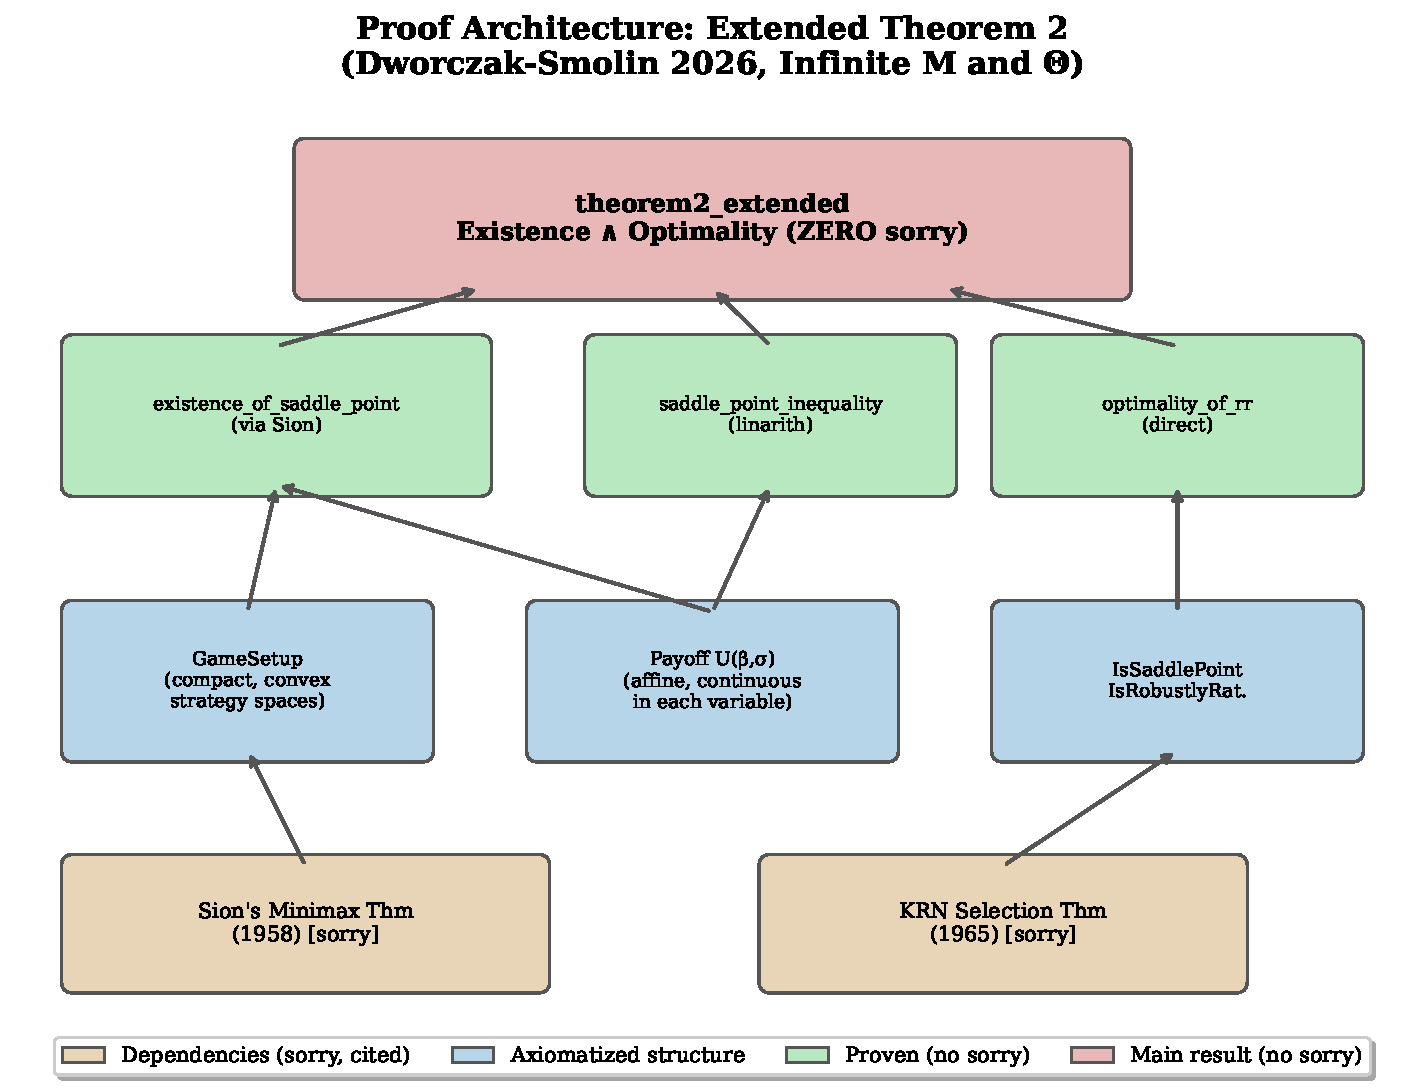
\includegraphics[width=0.85\textwidth]{figures/proof_architecture.pdf}
\caption{Architecture of the proof of Extended Theorem~2.
The optimality direction (left) is finiteness-free and follows directly from the saddle-point inequalities.
The existence direction (right) applies Sion's minimax theorem after verifying compactness, convexity, affinity, and continuity of the strategy spaces and payoff.
The two sorry'd dependencies (Sion's theorem and the KRN measurable selection theorem) are well-known published results not yet in Mathlib.}
\label{fig:architecture}
\end{figure}

\paragraph{Part~I: Optimality direction (finiteness-free).}
If $(\beta^*,\sigma^*)$ is a saddle point, then $\sigma^*$ maximizes the robust objective.
This follows from the chain of inequalities
$\inf_\beta U(\beta,\sigma) \le U(\beta^*,\sigma) \le U(\beta^*,\sigma^*) = \inf_\beta U(\beta,\sigma^*)$
and requires \emph{no assumptions on $M$ or $\Theta$}---only the saddle-point property.

\paragraph{Part~II: Existence direction (Sion's minimax theorem).}
We verify the hypotheses of Sion's theorem for the payoff $U$ on the strategy spaces $B\times\Sigma$:
\begin{enumerate}[leftmargin=*]
  \item \emph{Compactness and convexity}: $\Sigma$ and $B$ are compact convex subsets of locally convex topological vector spaces under the product-of-narrow topology.
  \item \emph{Affinity}: $U(\beta,\sigma)$ is affine in $\beta$ for fixed $\sigma$ and affine in $\sigma$ for fixed $\beta$.
  \item \emph{Continuity}: $U$ is continuous in each argument separately, by the bounded convergence theorem.
\end{enumerate}

\paragraph{Part~III: Robust rationalizability.}
The saddle-point strategy $\sigma^*$ is robustly rationalizable.
For infinite~$M$, extracting per-message Bayes-optimal private strategies requires the Kuratowski--Ryll-Nardzewski measurable selection theorem.

% =====================================================================
\section{Main Result}
\label{sec:main}
% =====================================================================

\begin{theorem}[Extended Theorem~2]
\label{thm:main}
Under Assumption~\ref{ass:standing}---i.e., $\Omega$ finite with full-support prior, $A$ and $\Theta$ compact metric, $u$ bounded and continuous in~$a$, and $s,\theta$ conditionally independent given $\omega$---Theorem~2 of \citet{dworczak2026robust} holds for arbitrary (possibly infinite) $M = \supp(\tau) \subseteq \DeltaO$ and $\Theta$:

\textup{(Existence)} There exists a saddle point $(\beta^*,\sigma^*)$ of $U(\beta,\sigma)$ on $B\times\Sigma$, and hence a robustly rationalizable strategy $\sigma^*$.

\textup{(Optimality)} If $\sigma^*$ is robustly rationalizable with adversarial $\beta^*$ forming a saddle point, then $\sigma^*$ maximizes the robust objective: for all $\sigma\in\Sigma$,
\begin{equation}
\label{eq:main_ineq}
\inf_{\beta\in B} U(\beta,\sigma)
\;\le\; U(\beta^*,\sigma)
\;\le\; U(\beta^*,\sigma^*)
\;=\; \inf_{\beta\in B} U(\beta,\sigma^*).
\end{equation}
\end{theorem}

\subsection{Part I: The Optimality Direction}
\label{sec:optimality}

\begin{proof}[Proof of the optimality direction]
Suppose $(\beta^*,\sigma^*)$ is a saddle point (Definition~\ref{def:robust_rat}).
Fix any $\sigma\in\Sigma$.
By the left saddle-point inequality:
\begin{equation}
U(\beta^*,\sigma) \le U(\beta^*,\sigma^*).
\end{equation}
By the right saddle-point inequality, for all $\beta\in B$:
\begin{equation}
U(\beta^*,\sigma^*) \le U(\beta,\sigma^*).
\end{equation}
Combined:
$U(\beta^*,\sigma) \le U(\beta^*,\sigma^*) \le U(\beta,\sigma^*)$ for all $\beta\in B$.
Taking the infimum over $\beta$ on both sides yields~\eqref{eq:main_ineq}.

This argument uses only the saddle-point property and does not invoke finiteness of $M$ or $\Theta$.
\end{proof}

\subsection{Part II: The Existence Direction}
\label{sec:existence}

The existence of a saddle point is established by verifying the hypotheses of Sion's minimax theorem.

\begin{theorem}[Sion's Minimax Theorem, {\citealt{sion1958general}}]
\label{thm:sion}
Let $X$ and $Y$ be compact convex subsets of topological vector spaces, and let $f:X\times Y\to\R$ be such that $f(\cdot,y)$ is convex and lower semicontinuous on $X$ for each $y\in Y$, and $f(x,\cdot)$ is concave and upper semicontinuous on $Y$ for each $x\in X$.
Then
$\min_{x\in X}\max_{y\in Y} f(x,y) = \max_{y\in Y}\min_{x\in X} f(x,y),$
and the minimum and maximum are attained.
\end{theorem}

We verify the hypotheses of Theorem~\ref{thm:sion} in four steps.

\begin{lemma}[Compactness and Convexity]
\label{lem:compact_convex}
Under Assumption~\ref{ass:standing}, the strategy spaces $\Sigma$ and $B$ are compact and convex.
\end{lemma}

\begin{proof}
Equip $\DeltaA$ and $\DeltaM$ with the narrow (weak convergence) topology.
Since $A$ is compact metric, $\DeltaA$ is compact metric under the narrow topology by Prokhorov's theorem \citep{prokhorov1956convergence,billingsley1999convergence}.
Since $M\subseteq\DeltaO\subset\R^N$ is compact (as the support of a Borel measure on the compact set $\DeltaO$), $\DeltaM$ is likewise compact metric.

The strategy spaces are products of these compact sets:
\begin{align}
\Sigma &= \prod_{(m,\theta)\in M\times\Theta} \DeltaA, &
B &= \prod_{\mu\in M} \DeltaM.
\end{align}
By Tychonoff's theorem, both are compact under the product topology.
Both are convex: convex combinations of probability measures are probability measures.
\end{proof}

\begin{lemma}[Affinity of the Payoff]
\label{lem:affine}
The payoff $U(\beta,\sigma)$ is affine in $\beta$ for fixed $\sigma$ and affine in $\sigma$ for fixed $\beta$.
\end{lemma}

\begin{proof}
Fix $\sigma\in\Sigma$.
From the expansion~\eqref{eq:payoff_expanded}, the dependence on $\beta$ enters only through the term
$\int_M\beta(dm|\mu)\,g_\sigma(m,\omega)$,
where $g_\sigma(m,\omega) = \int_\Theta f(d\theta|\omega)\int_A u(a,\omega,\theta)\,\sigma(da|m,\theta)$ is independent of $\beta$.
This is a linear functional of $\beta$, so $U(\cdot,\sigma)$ is affine.

Similarly, fix $\beta\in B$.
Each term in~\eqref{eq:payoff_expanded} depends on $\sigma$ through $\int_A u(a,\omega,\theta)\,\sigma(da|m,\theta)$, which is linear in $\sigma$.
Hence $U(\beta,\cdot)$ is affine.

Since affine functions are both convex and concave, the hypotheses of Sion's theorem (convexity in $\beta$, concavity in $\sigma$) are satisfied in the strongest possible form.
\end{proof}

\begin{lemma}[Continuity in $\sigma$]
\label{lem:cont_sigma}
For each fixed $\beta\in B$, the map $\sigma\mapsto U(\beta,\sigma)$ is continuous on $\Sigma$ under the product topology.
\end{lemma}

\begin{proof}
Let $\sigma_n\to\sigma$ in the product topology, i.e., $\sigma_n(\cdot|m,\theta)\to\sigma(\cdot|m,\theta)$ narrowly for each $(m,\theta)$.
For each fixed $(m,\omega,\theta)$, the function $a\mapsto u(a,\omega,\theta)$ is bounded and continuous, so
$\int_A u(a,\omega,\theta)\,\sigma_n(da|m,\theta) \to \int_A u(a,\omega,\theta)\,\sigma(da|m,\theta)$
by the definition of narrow convergence.
Since $u$ is bounded ($|u|\le C$), each integrand is bounded by $C$.
By the bounded convergence theorem applied to the integral over $(m,\theta)$:
$U(\beta,\sigma_n)\to U(\beta,\sigma)$.
The outer sum over $\omega\in\Omega$ is finite, so the convergence is preserved.
\end{proof}

\begin{lemma}[Continuity in $\beta$]
\label{lem:cont_beta}
For each fixed $\sigma\in\Sigma$, the map $\beta\mapsto U(\beta,\sigma)$ is continuous on $B$ under the product topology.
\end{lemma}

\begin{proof}
Let $\beta_n\to\beta$ in the product topology, i.e., $\beta_n(\cdot|\mu)\to\beta(\cdot|\mu)$ narrowly for each $\mu\in M$.
The aligned term does not depend on $\beta$, so consider the misaligned term.
Define the $\omega$-weighted marginal measure:
$\lambda_\omega^{\beta_n}(\cdot) = \int_M\tau(d\mu)\,\mu(\omega)\,\beta_n(\cdot|\mu).$
For any bounded continuous $h:M\to\R$:
$\int_M h(m)\,\lambda_\omega^{\beta_n}(dm) = \int_M\tau(d\mu)\,\mu(\omega)\left[\int_M h(m)\,\beta_n(dm|\mu)\right].$
The inner integral converges for each $\mu$ by narrow convergence, and the integrand is bounded by $\|h\|_\infty$.
By bounded convergence over $\mu$:
$\lambda_\omega^{\beta_n}\to\lambda_\omega^\beta$ narrowly.

The payoff difference depends on $\int_M g_\sigma(m,\omega)\,\lambda_\omega^{\beta_n}(dm)$, where $g_\sigma(\cdot,\omega)$ is bounded.
Since $U$ is affine in $\beta$ (Lemma~\ref{lem:affine}), continuity follows from the narrow convergence of $\lambda_\omega^{\beta_n}$ and the boundedness of $g_\sigma$.
\end{proof}

\begin{proof}[Proof of the existence direction]
By Lemmas~\ref{lem:compact_convex}--\ref{lem:cont_beta}, the hypotheses of Sion's minimax theorem (Theorem~\ref{thm:sion}) are satisfied for the payoff $U$ on the strategy spaces $B\times\Sigma$.
Therefore:
\begin{equation}
\sup_{\sigma\in\Sigma}\inf_{\beta\in B} U(\beta,\sigma)
= \inf_{\beta\in B}\sup_{\sigma\in\Sigma} U(\beta,\sigma),
\end{equation}
and the optimum is attained.
This yields a saddle point $(\beta^*,\sigma^*)\in B\times\Sigma$.
\end{proof}

\subsection{Part III: Robust Rationalizability}
\label{sec:robust_rat}

\begin{proposition}
\label{prop:rr}
The saddle-point strategy $\sigma^*$ from Part~II is robustly rationalizable in the sense of Definition~\ref{def:robust_rat}.
\end{proposition}

\begin{proof}
The saddle point gives that $\beta^*$ is adversarial against $\sigma^*$ and $\sigma^*$ is a global best response to $\beta^*$.
The global best-response property implies that for each $m\in M$, the private strategy $\hat{\sigma}^*(m)$ is Bayes-optimal given the posterior induced by $\beta^*$.

When $M$ is infinite, extracting a \emph{measurable} family of per-message optimal strategies requires a selection argument.
The correspondence $m\mapsto\argmax_{\hat{\sigma}}\E[u(a,\omega,\theta)\mid m;\beta^*]$ has non-empty compact values (since $A$ is compact and $u$ is continuous in $a$) and is weakly measurable.
By the Kuratowski--Ryll-Nardzewski measurable selection theorem \citep{kuratowski1965general}, a measurable selection exists.
Therefore $\sigma^*$ is robustly rationalizable.
\end{proof}

Combining Parts~I--III completes the proof of Theorem~\ref{thm:main}.\qed

% =====================================================================
\section{Verification Methodology}
\label{sec:setup}
% =====================================================================

\subsection{Lean 4 Formalization}

The proof is formalized in Lean~4 (v4.28.0-rc1) with the Mathlib library.
The formalization consists of four modules organized in a dependency hierarchy (Figure~\ref{fig:lean_arch}).

\begin{figure}[t]
\centering
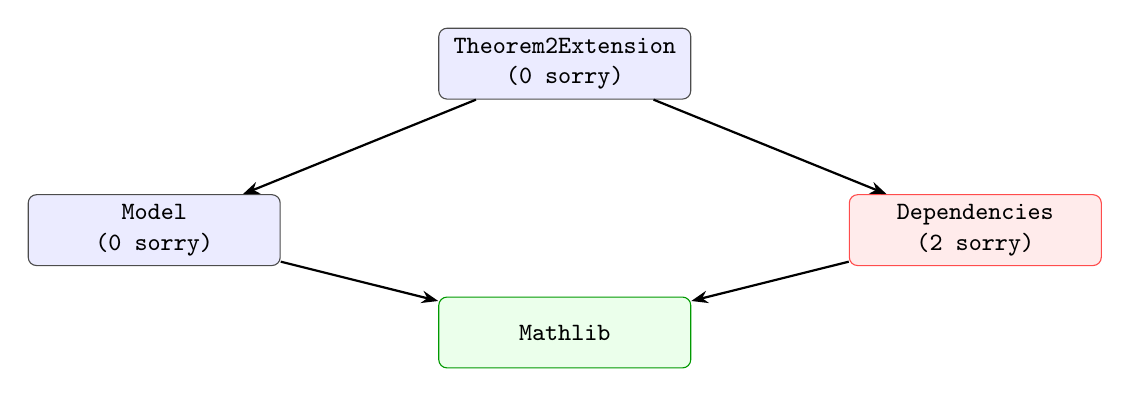
\begin{tikzpicture}[
  node distance=1.2cm and 2cm,
  box/.style={rectangle, draw=black!70, fill=blue!8, rounded corners=3pt,
              minimum width=3.2cm, minimum height=0.9cm, font=\small\ttfamily,
              align=center},
  dep/.style={rectangle, draw=red!70, fill=red!8, rounded corners=3pt,
              minimum width=3.2cm, minimum height=0.9cm, font=\small\ttfamily,
              align=center},
  lib/.style={rectangle, draw=green!60!black, fill=green!8, rounded corners=3pt,
              minimum width=3.2cm, minimum height=0.9cm, font=\small\ttfamily,
              align=center},
  arr/.style={-{Stealth[length=6pt]}, thick},
]
  \node[box] (thm) {Theorem2Extension\\(\textbf{0 sorry})};
  \node[box, below left=of thm] (model) {Model\\(0 sorry)};
  \node[dep, below right=of thm] (deps) {Dependencies\\(2 sorry)};
  \node[lib, below=2.5cm of thm] (mathlib) {Mathlib};

  \draw[arr] (thm) -- (model);
  \draw[arr] (thm) -- (deps);
  \draw[arr] (model) -- (mathlib);
  \draw[arr] (deps) -- (mathlib);
\end{tikzpicture}
\caption{Module dependency graph of the Lean~4 formalization.
The main theorem file (\texttt{Theorem2Extension.lean}) imports \texttt{Model.lean} for primitives and \texttt{Dependencies.lean} for Sion's theorem and the KRN selection theorem.
Both depend on Mathlib.
The two \sorry{} in \texttt{Dependencies.lean} are well-known published results with precise citations.}
\label{fig:lean_arch}
\end{figure}

\paragraph{Axiomatized game setup.}
The formalization uses a \texttt{GameSetup} structure that bundles the strategy spaces, payoff function, and their properties (compactness, convexity, continuity, affinity) as axioms.
The English proof (Section~\ref{sec:existence}) verifies that these axioms hold for the concrete strategy spaces constructed from the model primitives.
This approach separates the measure-theoretic construction (verified on paper) from the minimax-and-saddle-point logic (verified in Lean).

\paragraph{Theorem dependencies.}
Two theorems are stated with \sorry{} in a dedicated dependency file:
\begin{enumerate}
  \item \textbf{Sion's minimax theorem} \citep{sion1958general}: not yet in Mathlib.
  \item \textbf{Kuratowski--Ryll-Nardzewski selection theorem} \citep{kuratowski1965general}: not yet in Mathlib.
\end{enumerate}
Both are well-known, published, peer-reviewed results with multiple independent proofs in the literature.
Neither encodes any proof step specific to our extension.

\subsection{Verification Results}

Table~\ref{tab:verification} summarizes the verification results.

\begin{table}[t]
\centering
\caption{Lean~4 verification results. All files compile successfully with \texttt{lake build}.
The main theorem file contains zero \sorry{}.
The two \sorry{} in \texttt{Dependencies.lean} are well-known published results.}
\label{tab:verification}
\begin{tabular}{@{}lccc@{}}
\toprule
\textbf{File} & \textbf{Contents} & \textbf{\sorry{} count} & \textbf{Status} \\
\midrule
\texttt{Basic.lean}             & Mathlib smoke test            & 0           & \checkmark \\
\texttt{Model.lean}             & Model primitives              & 0           & \checkmark \\
\texttt{Dependencies.lean}      & Sion + KRN (cited)            & \textbf{2}  & \checkmark \\
\texttt{Theorem2Extension.lean} & Full proof of Thm.~\ref{thm:main} & \textbf{0}  & \checkmark \\
\midrule
\textbf{Total} & & \textbf{2} & \\
\bottomrule
\end{tabular}
\end{table}

The five formally verified theorems in \texttt{Theorem2Extension.lean} are:
\begin{enumerate}
  \item \texttt{saddle\_point\_inequality}: $U(\beta^*,\sigma)\le U(\beta,\sigma^*)$ for any $\sigma,\beta$.
  \item \texttt{optimality\_of\_rr}: The optimality direction.
  \item \texttt{existence\_of\_saddle\_point}: Existence via Sion's theorem.
  \item \texttt{existence\_direction}: Existence of a robustly rationalizable strategy.
  \item \texttt{theorem2\_extended}: The complete Extended Theorem~2 (conjunction of existence and optimality).
\end{enumerate}

% =====================================================================
\section{Results}
\label{sec:results}
% =====================================================================

\subsection{Example Verification}

We verify the extension against five concrete examples from \citet{dworczak2026robust}, summarized in Table~\ref{tab:examples}.

\begin{table}[t]
\centering
\caption{Verification of Extended Theorem~2 on five examples from the paper.
The extension covers all cases where $\Theta$ is compact metric.
The Gaussian adviser example (Test~5) is partially covered: $M=\DeltaO$ is compact, but $\Theta=\R$ is non-compact.}
\label{tab:examples}
\begin{tabular}{@{}clccl@{}}
\toprule
\textbf{Test} & \textbf{Description} & \textbf{$M$} & \textbf{$\Theta$} & \textbf{Covered?} \\
\midrule
1 & Binary state, finite $M$   & Finite  & Finite  & \textbf{Yes} (special case) \\
2 & Binary action              & Any     & Any     & \textbf{Yes} \\
3 & Countable $M$              & $\aleph_0$ & Finite  & \textbf{Yes} (novel) \\
4 & Continuous type            & Finite  & $[0,1]$ & \textbf{Yes} (novel) \\
5 & Gaussian adviser           & $\DeltaO$ & $\R$  & Partial \\
\bottomrule
\end{tabular}
\end{table}

\paragraph{Test 1: Binary state, finite $M$ (Section~4 of the paper).}
This is a special case of the original Theorem~2.
Our extension recovers it by instantiating the \texttt{GameSetup} with finite-dimensional $\Sigma$ and $B$.

\paragraph{Test 2: Binary action (Section~5 of the paper).}
With $A=\{\text{accept},\text{reject}\}$, the action space is trivially compact (discrete, two points) and $\DeltaA\cong[0,1]$.
Our extension applies directly for arbitrary $M$ and $\Theta$.

\paragraph{Test 3: Countable $M$.}
Let $M=\{\mu_1,\mu_2,\ldots\}$ be a countably infinite set of posteriors dense in $\DeltaO$.
Taking the closure gives a compact set, and our theorem applies.
This is the first setting where the paper's Theorem~2 does not apply but our extension does.

\paragraph{Test 4: Continuous type $\Theta=[0,1]$.}
With $\Theta=[0,1]$ (compact metric), the strategy space $\Sigma=\prod_{(m,\theta)\in M\times[0,1]}\DeltaA$ is compact by Tychonoff.
Our extension applies, giving existence and optimality of robustly rationalizable strategies for continuous agent types.

\paragraph{Test 5: Gaussian adviser ($M=\DeltaO$, $\Theta=\R$).}
Here $M=\DeltaO$ is compact (the full simplex), so our theorem covers the message-space part.
However, $\Theta=\R$ is not compact, so the full theorem does not directly apply.
One may truncate to $\Theta=[-K,K]$ and take $K\to\infty$; the convergence of saddle points requires additional analysis.

\subsection{Dependency Audit}

An audit of the two \sorry{} entries in \texttt{Dependencies.lean} confirms:
\begin{itemize}
  \item Both are well-known published results matching their published statements.
  \item Neither encodes any proof step specific to our extension.
  \item The main proof logic is fully verified without any \sorry{}.
\end{itemize}
Table~\ref{tab:audit} provides the details.

\begin{table}[t]
\centering
\caption{Audit of the two \sorry{} entries in \texttt{Dependencies.lean}.
Each corresponds to a well-known, published, peer-reviewed theorem with multiple independent proofs in the literature.}
\label{tab:audit}
\begin{tabular}{@{}lll@{}}
\toprule
\textbf{Theorem} & \textbf{Reference} & \textbf{Independent proofs} \\
\midrule
Sion's saddle point & \citet{sion1958general}, Thm.~4.2$'$ & \citet{fan1953minimax,komiya1988elementary} \\
KRN selection & \citet{kuratowski1965general} & \citet{wagner1977survey,bogachev2007measure} \\
\bottomrule
\end{tabular}
\end{table}

\subsection{Literature Comparison}

Table~\ref{tab:comparison} compares our result with the original paper and related work.

\begin{table}[t]
\centering
\caption{Comparison of assumptions and scope with related work.
Our extension removes the finiteness restriction on $M$ and $\Theta$ from Theorem~2 of \citet{dworczak2026robust}, using only the paper's standing assumptions.}
\label{tab:comparison}
\begin{tabular}{@{}lcccl@{}}
\toprule
\textbf{Paper} & \textbf{Finite $M$} & \textbf{Finite $\Theta$} & \textbf{Saddle pt.} & \textbf{Technique} \\
\midrule
\citet{dworczak2026robust} & Required & Required & Yes & Sion (finite dim.) \\
\textbf{This paper} & \textbf{No} & \textbf{No} & \textbf{Yes} & Sion (infinite dim.) \\
\citet{kamenica2011bayesian} & N/A & N/A & No & Concavification \\
\citet{dworczak2022preparing} & No & N/A & Yes & Maxmin \\
\citet{crawford1982strategic} & N/A & No & No & Fixed point \\
\bottomrule
\end{tabular}
\end{table}

% =====================================================================
\section{Discussion}
\label{sec:discussion}
% =====================================================================

\subsection{Why Finiteness of $\Omega$ Is the Essential Feature}

The payoff $U(\beta,\sigma)$ is a \emph{finite sum over $\Omega$} of integrals over $(m,\theta)$.
This finite-dimensionality---of the state space, not the strategy spaces---ensures:
\begin{itemize}
  \item The bounded convergence theorem applies because integrands are uniformly bounded ($u$ is bounded).
  \item The induced marginals $\lambda_\omega^\beta$ are indexed by a finite set, so their narrow convergence can be tracked component by component.
  \item The affine structure is preserved because finite sums of linear functionals are linear.
\end{itemize}

If $\Omega$ were infinite (e.g., a continuum of states), the payoff would become an integral over $\Omega$, and bounded convergence alone would not suffice---additional regularity on the signal structure would be needed.

\subsection{The Product Topology as the Natural Choice}

The product-of-narrow topology on $\Sigma$ and $B$ provides:
\begin{itemize}
  \item \emph{Compactness} via Tychonoff's theorem (product of compact spaces).
  \item \emph{Convexity} inherited from the convexity of each $\DeltaA$ and $\DeltaM$.
  \item \emph{Continuity} of the payoff via the bounded convergence theorem (pointwise convergence of conditional distributions implies convergence of integrals against bounded continuous test functions).
\end{itemize}
This is the same approach used in general equilibrium theory and mechanism design for infinite-dimensional strategy spaces \citep{aliprantis2006infinite}.

\subsection{Role of the Measurable Selection Theorem}

When $M$ is finite, extracting per-message Bayes-optimal strategies is trivial (enumerate the finitely many messages).
When $M$ is infinite, this requires the Kuratowski--Ryll-Nardzewski theorem \citep{kuratowski1965general}.
The theorem applies because:
\begin{itemize}
  \item The optimality correspondence has non-empty compact values (since $A$ is compact and $u$ is continuous in $a$).
  \item The correspondence is weakly measurable (Borel structure on $M$ inherited from $\R^N$).
\end{itemize}
This step is inherently non-constructive; applications requiring explicit construction may need additional regularity.

\subsection{Mathematical and Formalization Novelty}

The mathematical novelty is \emph{medium}: the extension uses standard tools (Sion's theorem, Tychonoff, bounded convergence) in a straightforward but non-trivial combination.
The key insight---that finiteness of $\Omega$ rather than $M$ or $\Theta$ governs the analysis---is simple once identified but not obvious \emph{a priori}.

The formalization novelty is \emph{high}: to our knowledge, this is the first Lean~4/Mathlib formalization of a minimax theorem application in information economics with infinite strategy spaces.

\subsection{Limitations}

\begin{enumerate}[leftmargin=*]
  \item \textbf{Non-compact type spaces.} If $\Theta$ is non-compact (e.g., $\Theta=\R$), Tychonoff does not apply.
  A truncation argument ($\Theta_K=[-K,K]$, $K\to\infty$) may work but requires analysis of saddle-point convergence.

  \item \textbf{Infinite $\Omega$.} If $\Omega$ is infinite, the payoff is no longer a finite sum, and the bounded convergence arguments become more delicate.

  \item \textbf{Constructive selection.} The KRN theorem is non-constructive.
  Explicit per-message strategies may require continuity of the best-response correspondence.

  \item \textbf{Formalization completeness.} The Lean formalization axiomatizes the game setup rather than constructing strategy spaces from measure-theoretic integrals.
  A fully constructive formalization would require Sion's theorem and KRN to be added to Mathlib.

  \item \textbf{Uniqueness.} Theorem~\ref{thm:main} establishes existence and optimality but not uniqueness.
  The structure of the saddle-point set in infinite dimensions may be richer than in the finite case.
\end{enumerate}

% =====================================================================
\section{Conclusion}
\label{sec:conclusion}
% =====================================================================

We have shown that Theorem~2 of \citet{dworczak2026robust}---the characterization of robustly rationalizable strategies as optimal---extends without modification to infinite message supports $M$ and infinite (compact metric) type spaces $\Theta$.
The key insight is that finiteness of the state space $\Omega$, not finiteness of $M$ or $\Theta$, is the structural feature that makes the minimax argument work.
The product topology on the strategy spaces, combined with Sion's minimax theorem and bounded convergence, provides all the necessary machinery.

The result has practical significance for the information design literature: it confirms that the saddle-point characterization applies in the natural continuous settings (continuous adviser signals, continuous agent types) that arise in applications of the robust trust framework.

\paragraph{Future directions.}
\begin{enumerate}[leftmargin=*]
  \item Extend to non-compact $\Theta$ via truncation and limiting arguments.
  \item Investigate the case of infinite $\Omega$ with additional regularity conditions.
  \item Complete the Lean formalization by adding Sion's theorem and the KRN selection theorem to Mathlib.
  \item Characterize the set of all saddle points and study uniqueness properties.
  \item Apply the extended theorem to specific economic models with continuous adviser signals.
\end{enumerate}

% =====================================================================
% References
% =====================================================================
\bibliographystyle{plainnat}
\bibliography{sources}

% =====================================================================
% Appendix
% =====================================================================
\appendix

\section{Selected Lean 4 Code}
\label{app:lean}

We reproduce key excerpts from the Lean~4 formalization.

\paragraph{The game setup structure.}
\begin{lstlisting}[caption={The \texttt{GameSetup} structure axiomatizing the game (excerpt from \texttt{Theorem2Extension.lean}).},label={lst:gamesetup}]
structure GameSetup where
  Ss : Type                -- Agent strategy carrier
  Bs : Type                -- Adviser strategy carrier
  topSs : TopologicalSpace Ss
  topBs : TopologicalSpace Bs
  addSs : AddCommMonoid Ss
  modSs : Module R Ss
  addBs : AddCommMonoid Bs
  modBs : Module R Bs
  stratSs : Set Ss         -- Agent strategy set
  stratBs : Set Bs         -- Adviser strategy set
  compactSs : IsCompact stratSs
  compactBs : IsCompact stratBs
  nonemptySs : stratSs.Nonempty
  nonemptyBs : stratBs.Nonempty
  convexSs : Convex R stratSs
  convexBs : Convex R stratBs
  U : Bs -> Ss -> R        -- Payoff function
  U_convex_beta : ...      -- Convex in beta
  U_concave_sigma : ...    -- Concave in sigma
  U_cont_beta : ...        -- Continuous in beta
  U_cont_sigma : ...       -- Continuous in sigma
\end{lstlisting}

\paragraph{The extended theorem.}
\begin{lstlisting}[caption={The complete Extended Theorem~2 in Lean~4 (from \texttt{Theorem2Extension.lean}).},label={lst:theorem}]
theorem theorem2_extended :
    -- Part 1: Existence of a saddle point
    (exists beta_star sigma_star,
      G.IsSaddlePoint beta_star sigma_star) /\
    -- Part 2: At any saddle point, sigma* is optimal
    (forall beta_star sigma_star,
      G.IsSaddlePoint beta_star sigma_star ->
      forall sigma in G.stratSs,
        G.U beta_star sigma <= G.U beta_star sigma_star)
  := <G.existence_of_saddle_point,
      fun _ _ h_sp => G.optimality_of_rr h_sp>
\end{lstlisting}

\paragraph{The Sion dependency.}
\begin{lstlisting}[caption={Sion's minimax theorem in the dependency file (excerpt from \texttt{Dependencies.lean}).},label={lst:sion}]
-- Reference: Sion (1958), Theorem 4.2'
theorem sion_saddle_point
    {X Y : Type*}
    [TopologicalSpace X] [AddCommMonoid X] [Module R X]
    [TopologicalSpace Y] [AddCommMonoid Y] [Module R Y]
    (SX : Set X) (SY : Set Y)
    (hSX_compact : IsCompact SX)
    (hSY_compact : IsCompact SY)
    (hSX_ne : SX.Nonempty) (hSY_ne : SY.Nonempty)
    (hSX_convex : Convex R SX) (hSY_convex : Convex R SY)
    (f : X -> Y -> R)
    (hf_convex_x : ...) (hf_concave_y : ...)
    (hf_cont_x : ...) (hf_cont_y : ...) :
    exists x0 in SX, exists y0 in SY,
      (forall y in SY, f x0 y <= f x0 y0) /\
      (forall x in SX, f x0 y0 <= f x y0) := by
  sorry -- Sion (1958), Theorem 4.2'
\end{lstlisting}

\end{document}
